\documentclass{exercise}

\institute{Applied and Computational Mathematics}
\title{Selbstrechenübung 7}
\author{Joshua Feld, 406718}
\course{Mathematische Grundlagen IV}
\professor{Torrilhon \& Berkels}
\semester{Sommersemester 2022}
\program{CES (Bachelor)}

\begin{document}
    \maketitle


    \section*{Aufgabe 1}
    
    \begin{problem}
        \emph{Laut ADAC bildeten sich auf den deutschen Autobahnen im Jahr 2009 pro Tag Staus mit einer durchschnittlichen Länge von \(1000\sis{\kilo\meter}\).
        Um ein Straßennetzwerk effizient auslasten zu können, muss das Verkehrsaufkommen auf den Straßen möglichst realistisch simuliert werden.
        Ein einfaches eindimensionales Verkehrsfluss-Modell wird in dieser Aufgabe vorgestellt.}

        Die Anzahl der Fahrzeuge pro Länge wird Verkehrsdichte \(\rho\parentheses*{\hat{t}, \hat{x}}\) genannt, die vom Ort \(\hat{x}\) und der Zeit \(\hat{t}\) abhängt.
        Bezeichne \(v\parentheses*{\hat{x}}\) die Geschwindigkeit des Verkehrsflusses an der Stelle \(\hat{x}\) zum Zeitpunkt \(\hat{t}\), so lässt sich aus der Erhaltung der Fahrzeuge (also ohne Zu- und Abfahrten) die Gleichung
        \begin{equation}\label{eq:1}
            \frac{\partial\rho}{\partial\hat{t}} + \frac{\partial\parentheses*{\rho v}}{\partial\hat{x}} = 0
        \end{equation}
        herleiten.
        Diese Gleichung hat allerdings immernoch zwei unbekannte Funktionen und ist daher in dieser Form nicht lösbar.
        \begin{enumerate}
            \item Bei dem Lighthill-Whitham Modell nimmt man den Zusammenhang
            \[
                v\parentheses*{\rho} = v_{\text{max}}\parentheses*{1 - \frac{\rho}{\rho_{\text{max}}}}
            \]
            an, wobei \(v_{\text{max}}\) die Maximalgeschwindigkeit und \(\rho_{\text{max}}\) die Maximaldichte bezeichnen.
            Zeigen Sie durch geeignete Substitutionen, dass \eqref{eq:1} auf die \emph{Burgers'sche Gleichung}
            \[
                \frac{\partial u}{\partial t} + u \cdot \frac{\partial u}{\partial x} = 0
            \]
            umgeformt werden kann.
            Dabei sind \(u\), \(t\) und \(x\) dimensionslose Größen.
            \item Erstellen Sie ein \(t\)-\(x\)-Diagramm für den Verlauf der Charakteristiken der Burgers'schen Gleichung auf \(\Omega = \brackets*{-5, 5} \times \brackets*{0, 2}\) mit dem Anfangswert
            \[
                u\parentheses*{x, 0} = 1 + e^{-x^2}.
            \]
            Was bedeutet en Schnittpunkt zweier Charakteristiken für die Lösung?
        \end{enumerate}
    \end{problem}

    \subsection*{Lösung}
    \begin{enumerate}
        \item Der Einfachheit halber definieren wir
        \[
            f\parentheses*{\rho} := \rho \cdot v_{\text{max}}\parentheses*{1 - \frac{\rho}{\rho_{\text{max}}}}.
        \]
        Dann gilt
        \[
            0 = p_{\hat{t}} + \parentheses*{v \cdot \rho}_{\hat{x}} = \rho_{\hat{t}} + \parentheses*{f\parentheses*{\rho}}_{\hat{x}} = \rho_{\hat{t}} + f'\parentheses*{\rho} \cdot \rho_{\hat{x}}.
        \]
        Definiere
        \[
            u := 1 - \frac{2\rho}{\rho_{\text{max}}} \iff \rho = \frac{\rho_{\text{max}}}{2}\parentheses*{1 - u}, \quad x := \frac{\hat{x}}{L}, \quad t := \hat{t} \cdot \frac{v_{\text{max}}}{L},
        \]
        wobei \(L\) eine festgelegte Länge ist.
        Dann ist
        \begin{align*}
            \rho_{\hat{t}} &= \rho_t \frac{v_{\text{max}}}{L} = -\frac{\rho_{\text{max}}v_{\text{max}}}{2L}u_t,\\
            \rho_{\hat{x}} &= \rho_x \frac{1}{L} = \rho'\parentheses*{u}u_x \frac{1}{L} = -\frac{\rho_{\text{max}}}{2}u_x \frac{1}{L} = -\frac{\rho_{\text{max}}}{2L}u_x\\
            f'\parentheses*{\rho} = v_{\text{max}}\parentheses*{1 - \frac{2\rho}{\rho_{\text{max}}}}.
        \end{align*}
        Damit ergibt sich
        \[
            0 = \rho_{\hat{t}} + f'\parentheses*{\rho} \cdot \rho_{\hat{x}} = -\frac{\rho_{\text{max}}v_{\text{max}}}{2L}u_t - \frac{\rho_{\text{max}}}{2L}u_x \cdot v_{\text{max}}\underbrace{\parentheses*{1 - \frac{2\rho}{\rho_{\text{max}}}}}_{= u} \iff 0 0 u_t + u \cdot u_x.
        \]
        \item Die Charakteristiken sind Lösungen von
        \begin{align*}
            \text{I.} \quad x'\parentheses*{s} &= z\parentheses*{s}, \quad s > 0, x\parentheses*{0} = x_0,\\
            \text{II.} \quad t'\parentheses*{s} &= 1, \quad s > 0, t\parentheses*{0} = 0 \implies t = 2,\\
            \text{III.} \quad z'\parentheses*{s} &= 0, \quad s > 0, z\parentheses*{0} = 1 + e^{-x_0^2} \implies z\parentheses*{s} = 1 + e^{-x_0^2}
            \xRightarrow{\text{I.}} x\parentheses*{s} &= \parentheses*{1 + e^{-x_0^2}} \cdot s + x_0\\
            \implies x\parentheses*{t} &= \parentheses*{1 + e^{-x_0^2}} \cdot t + x_0.
        \end{align*}
        \begin{center}
            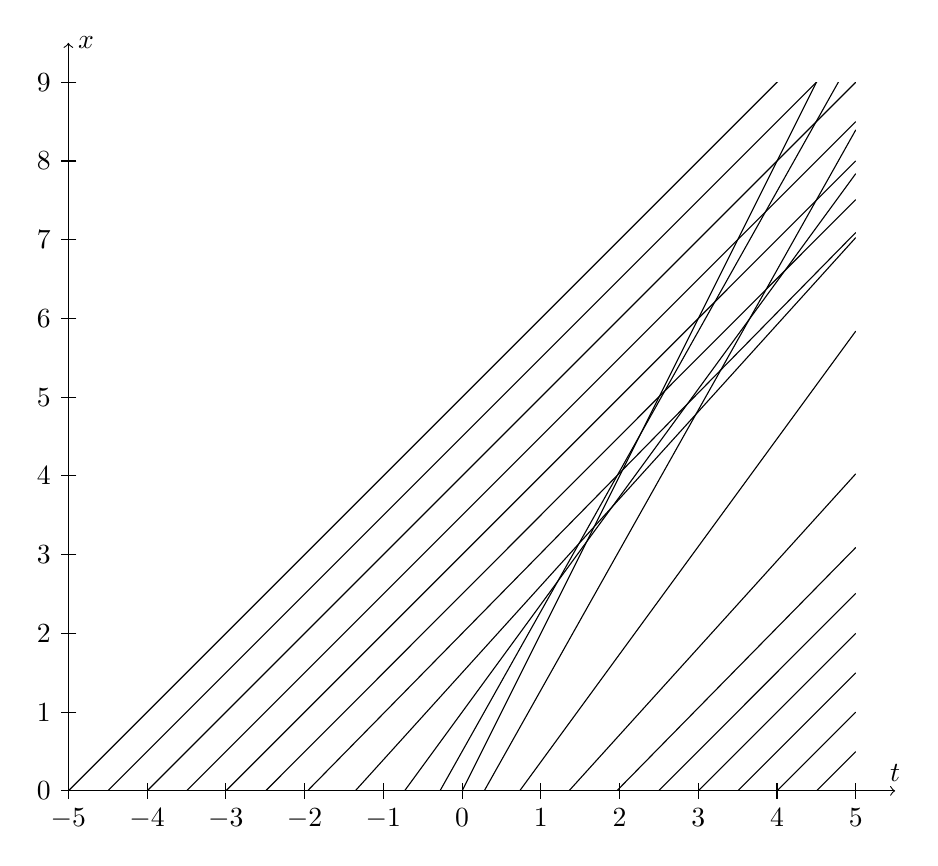
\begin{tikzpicture}
                \draw[->] (-5,0) -- (5.5,0) node[above] {\(t\)};
                \draw[->] (-5,0) -- (-5,9.5) node[right] {\(x\)};
                \foreach \i in {-5,-4,...,5}
                {
                    \draw (\i,.1) -- (\i,-.1) node[below] {\(\i\)};
                }
                \foreach \i in {0,1,...,9}
                {
                    \draw (-4.9,\i) -- (-5.1,\i) node[left] {\(\i\)};
                }
                \clip (-5,0) rectangle (5,9);
                \foreach \i in {-5,-4.5,...,5}
                {
                    \draw[domain=-5:5,smooth,variable=\t] plot ({\t},{\t+exp(-(\i*\i))*\t+\i});
                }
            \end{tikzpicture}
        \end{center}
        Charakteristiken sind nur bis zum ersten Schnitt mit einer weiteren Charakteristik gültig.
        Da die Lösung auf Charakteristiken konstant ist, bedeutet ein Schnitt zweier Charakteristiken mit verschiedenen Funktionswerten eine Unstetigkeit der Lösung im Schnittpunkt.
    \end{enumerate}


    \section*{Aufgabe 2}
    
    \begin{problem}
        Wir betrachten das Poisson-Problem:
        \begin{align*}
            -\Delta u\parentheses*{x, y} &= f\parentheses*{x, y}, \quad \parentheses*{x, y} \in \Omega = \parentheses*{0, 1}^2,\\
            u\parentheses*{x, y} &= g\parentheses*{x, y}, \quad \parentheses*{x, y} \in \partial\Omega.
        \end{align*}
        Bestimmen Sie, ob für diese Probleme die Konvergenzaussagen aus der Vorlesung erfüllt sind:
        \begin{enumerate}
            \item Problem 1:
            \begin{align*}
                u\parentheses*{x, y} &= \parentheses*{1 - \parentheses*{2x - 1}^4}\parentheses*{\parentheses*{2y - 1}^2 - 1},\\
                f\parentheses*{x, y} &= 8 \cdot \parentheses*{24 \cdot \parentheses*{1 - 2x}^2\parentheses*{y - 1}y + \parentheses*{1 - 2x}^4 - 1},\\
                g\parentheses*{x, y} &= u\parentheses*{x, y}.
            \end{align*}
            \item Problem 2:
            \begin{align*}
                u\parentheses*{x, y} &= y^4\parentheses*{\frac{1}{6}x^3\log\parentheses*{x} - \frac{11x^3}{36}},\\
                f\parentheses*{x, y} &= \frac{1}{3}xy^2 \cdot \parentheses*{-3 \cdot \parentheses*{2x^2 + y^2}\log\parentheses*{x} + 11x^2 + 3y^2},\\
                g\parentheses*{x, y} &= u\parentheses*{x, y}.
            \end{align*}
        \end{enumerate}
    \end{problem}
    
    \subsection*{Lösung}
    \begin{enumerate}
        \item \(u\parentheses*{x, y} = a\parentheses*{x}b\parentheses*{y}\) ist das Produkt zweier Polynome in \(x\) bzw. \(y\).
        Somit ist schon \(u\parentheses*{x, y} \in C^4\parentheses*{\Omega}\) erfüllt.
        Für die vierten Ableitungen gilt
        \[
            \partial_x^4 u\parentheses*{x, y} = -384 \cdot \parentheses*{\parentheses*{2y - 1}^2 - 1}, \quad \partial_y^4 u\parentheses*{x, y} = 0.
        \]
        Damit folgt
        \[
            C = \norm*{\partial_x^4 u\parentheses*{x, y}}_{\infty, \bar{\Omega}} = 384 < \infty.
        \]
        Für Problem 1 kovergiert das Verfahren somit.
        \item Wir können zwar zeigen, dass \(u \in C^4\parentheses*{\Omega}\) gilt, jedoch ist die vierte Ableitung am Rand unbeschränkt:
        \[
            \frac{\partial^4 u}{\partial x^4}\parentheses*{x, y} = \frac{y^4}{x}.
        \]
        Daher gilt \(u \in C^4\parentheses*{\Omega}\) aber \(u \not\in C^4\parentheses*{\bar{\Omega}}\).
        Somit folgt
        \[
            \norm*{\frac{\partial^4 u}{\partial x^4}}_{L^\infty\parentheses*{\bar{\Omega}}} = \infty.
        \]
        Damit gilt die Konvergenzaussage aus der Vorlesung für Problem 2 nicht.
    \end{enumerate}


    \section*{Aufgabe 3}
    
    \begin{problem}
        Diskretisieren Sie das Konvektionsproblem
        \begin{align*}
            u'\parentheses*{x} &= f\parentheses*{x}, \quad x \in \Omega = \parentheses*{0, 1}, u \in C^2\parentheses*{\Omega},\\
            u\parentheses*{0} &= 0
        \end{align*}
        mit der einseitigen finiten Differenz
        \[
            u'\parentheses*{x} \approx \frac{u\parentheses*{x} - u\parentheses*{x - h}}{h}, \quad h = \frac{1}{n}, n \in \N
        \]
        und stellen Sie das zugehörige Gleichungssystem \(Au_h = b\) auf.
        Bestimmen Sie \(A^{-1}\) und \(\norm*{A^{-1}}_\infty\).
    \end{problem}
    
    \subsection*{Lösung}
    Sei \(h = \frac{1}{n}\), dann gibt es insgesamt \(n\) Gitterpunkte.
    Die Approximation von \(u_h\parentheses*{x}\) im Gitterpunkt \(x_j = jh\) sei \(u_j\).
    Dann gilt im Gitterpunkt \(x_1\)
    \[
        \frac{1}{h}u_1 = f_1 = f\parentheses*{x_1}
    \]
    und für \(j = 2, \ldots, n\)
    \[
        \frac{1}{h}\parentheses*{u_j - u_{j - 1}} = f\parentheses*{x_j} = f_j.
    \]
    Wir erhalten also das finite Differenzen Gleichungssystem
    \[
        Au_h = b
    \]
    mit
    \[
        A = \frac{1}{h}\begin{pmatrix}
            1 & 0 & \cdots & \cdots & 0\\
            -1 & \ddots & \ddots & & \vdots\\
            0 & \ddots & \ddots & \ddots & \vdots\\
            \vdots & \ddots & \ddots & \ddots & 0\\
            0 & \cdots & 0 & -1 & 1
        \end{pmatrix}, \quad u_h = \begin{pmatrix}
            u_1\\
            \vdots\\
            u_n
        \end{pmatrix}, \quad b = \begin{pmatrix}
            f_1\\
            \vdots\\
            f_n
        \end{pmatrix}.
    \]
    \(A^{-1}\) enthält in der Spalte \(j\) die Lösung des Gleichungssystems
    \[
        Ax = e_j,
    \]
    wobei \(e_j\) den \(j\)-ten Einheitsvektor bezeichne, d.h.
    \[
        Ax = e_j \iff \frac{1}{h}\begin{pmatrix}
            1 & 0 & \cdots & \cdots & 0\\
            -1 & \ddots & \ddots & & \vdots\\
            0 & \ddots & \ddots & \ddots & \vdots\\
            \vdots & \ddots & \ddots & \ddots & 0\\
            0 & \cdots & 0 & -1 & 1
        \end{pmatrix}\begin{pmatrix}
            x_1\\
            \vdots\\
            x_n
        \end{pmatrix} = \begin{pmatrix}
            0\\
            \vdots\\
            0\\
            1\\
            0\\
            \vdots\\
            0
        \end{pmatrix}.
    \]
    Aus Zeile 1 folgt \(x_1 = 0\).
    Aus den Zeilen \(k < j\) folgt
    \[
        \frac{1}{h}x_k = \frac{1}{h}x_{k - 1} \quad \text{bzw.} \quad x_k = x_{k - 1}.
    \]
    Es ist also \(x_k = 0\) für \(k < j\).
    Die \(j\)-te Zeile ergibt
    \[
        \frac{1}{h}x_j = 1 + \frac{1}{h}\underbrace{x_{j - 1}}_{= 0} \quad \text{bzw.} \quad x_j = h.
    \]
    Aus den Zeilen \(l > j\) folgt
    \[
        \frac{1}{h}x_l = \frac{1}{h}x_{l - 1} \quad \text{bzw.} \quad x_l = x_{l - 1}
    \]
    und es sind alle \(x_l = h\) für \(l > j\).
    Insgesamt ist dann
    \[
        x = \begin{pmatrix}
            0\\
            \vdots\\
            0\\
            h\\
            \vdots\\
            h
        \end{pmatrix}.
    \]
    Berechnet man so alle Spalten von \(A^{-1}\), erhält man
    \[
        A^{-1} = h\begin{pmatrix}
            1 & 0 & \cdots & 0\\
            \vdots & \ddots & \ddots & \vdots\\
            \vdots & & \ddots & 0\\
            1 & \cdots & \cdots & 1
        \end{pmatrix}.
    \]
    Die \(\norm*{A^{-1}}_\infty\)-Norm ist die größte Zeilensumme, also
    \[
        \norm*{A^{-1}}_\infty = hn = 1.
    \]
\end{document}
